\chapter{Fisher statistics}

BACKGROUND: 
read Taylor (1982), Chapters 1-5.  \nocite{taylor82}
\vskip 12pt



We have laid out the need for statistical analysis of paleomagnetic data in  the preceding chapters.
For instance, we require a method for determining a mean direction from a set of observations. Such a
method should provide some measure of uncertainty in the mean direction. Additionally, we need methods
for assessing the significance of field tests of paleomagnetic stability. In this chapter, we introduce basic statistical methods for analysis of
directional data. It is sometimes said that statistical analyses are used by
scientists in the same manner that a drunk uses a light pole: more for support than for illumination. Although
this might be true, statistical analysis is fundamental to any paleomagnetic investigation. An appreciation of
the basic statistical methods is required to understand paleomagnetism.

Most of the statistical methods used in paleomagnetism have direct analogies to ``planar'' statistics. We
begin by reviewing the basic properties of the 
\index{distributions!normal}
normal distribution.
This distribution is used for statistical analysis of a wide variety of observations and will be familiar to many
readers.  We then tackle statistical analysis of directional data  by analogy with the normal distribution. Although
the reader might not follow all aspects of the mathematical formalism, this is no cause for alarm.
Graphical displays of functions and examples of statistical analysis will provide the more important intuitive
appreciation for the statistics.

\section {The normal distribution}

Any statistical method for determining a mean (and confidence limit) from a set of observations is based on
a probability density function. This function describes the distribution of observations for a hypothetical,
infinite set of observations called a population. The Gaussian probability density function 
(normal distribution)
has the familiar bell-shaped form shown in Figure~\ref{fig:gauss}a.   The meaning of the probability density function
$f(z)$  is that the proportion of observations within an interval of incremental width $dz$  centered on $z$ is $f(z) dz$.

\begin{figure}[h!tb]
%\epsfxsize 13cm
%\centering \epsffile{EPSfiles/gauss.eps}
\centering  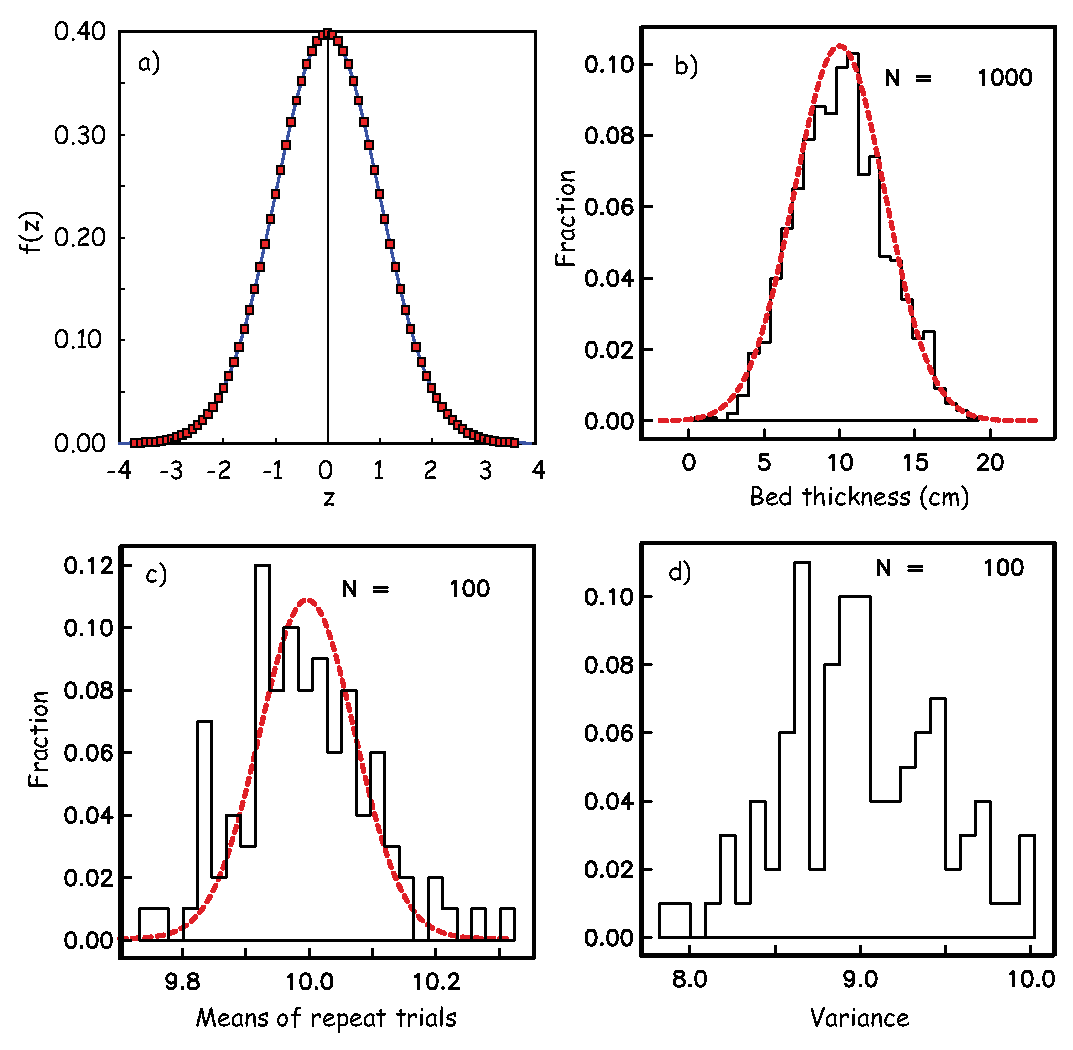
\includegraphics[width= 13 cm]{EPSfiles/gauss.eps}
\caption{a) The Gaussian probability density function
(normal distribution, Equation 11.1). The
proportion of observations within an interval $dz$
centered on $ z$ is $f(z)dz$.
b) Histogram of 1000 measurements of bed thickness in a sedimentary
formation. Also shown is the smooth curve of a normal distribution 
with a mean of 10 and a standard deviation of 3.  c) Histogram of the means from 100 repeated sets of 1000 measurements from the same sedimentary formation.  The distribution of the means is much tighter.  d) Histogram of the  variances ($s^2$) from the same set of experiments as in c).  The distribution of variances is not bell shaped; it is $\chi^2$. }
\label{fig:gauss}
\end{figure}
\clearpage

The 
\index{Gaussian!probability density function}
Gaussian probability density function  is given by:

\beq
{f(z)} = { 1\over{\sigma \sqrt{2\pi}}}{\exp {\bigl( {-z^2 \over 2 } \bigr)} },
\label{eq:normal}
\eeq
\noindent where

$$
z = { { x-\mu} \over {\sigma} }.
$$

\noindent
$x$ is the variable measured, $\mu$ is the true mean, and $\sigma$ is the standard deviation. The parameter $\mu$ determines
the value of $x$ about which the distribution is centered, while $\sigma$ determines the width of the distribution about
the true mean. By performing the required integrals (computing area under curve $f(z)$), it can be shown that
68\% of the readings in a normal distribution are within $\sigma$ of $\mu$, while 95\% are within 1.96$\sigma$ of $\mu$.

The usual situation is that one has made a finite number of measurements of a variable $x$. In the
literature of statistics, this set of measurements is referred to as a sample. Let us say that we made 1000 measurements of some parameter, say bed thickness (in cm)
in a particular sedimentary formation.  We plot these
in histogram form in Figure~\ref{fig:gauss}b. 

By using the methods of Gaussian
statistics, one is supposing that the observed sample has been drawn from a population of observations that
is normally distributed. The true mean and standard deviation of the population are, of course, unknown.
But the following methods allow estimation of these quantities from the observed sample.
A normal distribution can be characterized by two parameters, the mean
($\mu$) and  the variance $\sigma^2$.   How to estimate the parameters
of the underlying distribution is the art of statistics.  We all
know that the arithmetic mean of a batch of data $\bar x$ drawn from a normal distribution
is calculated by:
$$
{\bar x }= {1\over N} {\sum_{i=1}^N x_i},
$$
\noindent where $N$ is the number of measurements and $x_i$ is an individual measurement. 

The mean estimated from the data shown in Figure~\ref{fig:gauss}b is
10.09.  If we had measured an infinite number of bed thicknesses, we would have
gotten the bell curve shown  as  the dashed line  and calculated a mean of
10.  

The ``spread'' in the data is characterized by the
\index{variance}
 variance $\sigma^2$.
Variance for normal distributions can be estimated by the statistic
 $s^2$:

\begin{equation}
s^2 = {1\over {N-1}} \sum_{i=1}^N (x_i-\bar x)^2.
\label{eq:sigma}
\end{equation}


In order to get the units right on the spread about the mean (cm -- not cm$^2$), we have to take the 
square root of $s^2$.  The statistic $s$ gives an estimate of the 
standard deviation $\sigma$ and is the bounds around the mean that includes 
63\% of the values.  The 95\% confidence bounds are given by
1.96$s$ (this is what a ``2-$\sigma$ error'' is), and should include
95\% of the observations.
The bell curve shown in Figure~\ref{fig:gauss}b  has a $\sigma$ (standard deviation)
of 3, while the $s$ is  2.97.


If you repeat the bed measuring experiment
 a few times, you will never get exactly the same measurements in the different trials.  The mean and standard deviations measured
for each trial then are ``sample'' means and standard deviations.
If you plotted up all those sample means, you would get another
normal distribution whose mean should be pretty close to the 
true mean, but with a much more narrow standard deviation.  In Figure~\ref{fig:gauss}c we plot a histogram of  means from 100 such trials of 1000 measurements  each drawn from the same distribution of $\mu = 10, \sigma = 3$.  In general,
we expect the standard deviation of the means (or  
\index{standard error of the mean}
{\it standard error of the mean},  $s_m$)  to be related to $s$ by 
$$
s_m = {s\over {\sqrt{N_{trials}}}}.
$$

What if we were to plot up a histogram of  the estimated variances as in Figure~\ref{fig:gauss}c?
Are these also normally distributed?  The answer is 
no, because variance is a squared parameter relative to the 
original units.  In fact, the distribution of variance estimates
from normal distibutions is expected to be 
\index{distributions!chi-square}
{\it chi-squared}  ($\chi^2$). The width of the $\chi^2$ distribution is also governed by  how many measurements were made.  The so-called number of 
\index{degrees of freedom}
{\it degrees of freedom}  ($\nu$) is given by the number of measurements made
minus the number of measurements required to make the estimate, so
$\nu$ for our case is $N-1$.  Therefore we expect the 
variance estimates to follow a $\chi^2$ distribution with $N-1$ 
degrees of freedom of $\chi^2_{\nu}$.   


The estimated standard error of the mean, $s_m$, provides a confidence limit for the calculated mean. Of
all the possible samples that can be drawn from a particular normal distribution, 95\% have means, $\bar x$, within
2$s_m$ of $\bar x$. (Only 5\% of possible samples have means that lie farther than 2$s_m$ from $\bar x$.) Thus the 95\% confidence limit on the calculated mean, $\bar x$, is 2$s_m$, and we are 95\% certain that the true mean of the
population from which the sample was drawn lies within 2$s_m$ of $\bar x$.
The estimated standard error of the mean, $s_m$
 decreases 1/$\sqrt N$. Larger samples provide more precise estimations of the true mean;  this is reflected
in the smaller confidence limit with increasing $N$.


We often wish to consider ratios of variances  derived from normal distributions (for example
to decide if the data are more scattered in one data set relative
to another).  In order to do this, we must know what ratio would be 
expected from data sets drawn from the same distributions.  Ratios
of such variances follow a so-called 
\index{distributions!$F$}
$F$ distribution with $\nu_1$ and
$\nu_2$ degrees of freedom for the two data sets.  This is 
denoted $F[\nu_1,\nu_2]$.  Thus if the ratio $F$, given by:
$$
{F}={{s_1^2}\over {s_2^2}},
$$
\noindent
is greater than the 5\% critical value of $F[\nu_1,\nu_2]$ (check the
F distribution tables in your favorite statistics book or online), the 
hypothesis  that the two variances are the same can be rejected at the
95\% level of confidence.

A related test to the $F$ test  is 
\index{statistical tests!Student's $t$}
Student's $t$-test.  This test compares differences in normal data sets and provides a means for judging their significance.  Given two sets of measurements of bed thickness, for example in two different sections, the $t$ test addresses the likelihood that the difference between the two means is significant at a given level of probability.       If the estimated means and standard deviations of the two sets of $N_1$ and $N_2$ measurements are $\bar x_1,\sigma_1$ and $\bar x_2,\sigma_2$ respectively, the $t$ statistic can be calculated by:

$$
{t} = { {\bar x_1 - \bar x_2} \over {\sigma_{(x_1-x_2)} }},
$$
\noindent where
$$
 {\sigma_{(x_1-x_2)} } = \sqrt{ 
{ {(N_1-1)\sigma_1^2 + (N_2 -1)\sigma_2^2)}\over {\nu} }
{\bigl({ {1\over{N_1} }+ { {1\over{N_2} }\bigr) }}}
}.
$$
\noindent  Here $\nu= N_1+N_2 -2$.     If this number is below a critical value for $t$ then the null hypothesis that the two sets of data are the same cannot be rejected at a given level of confidence.  The critical value can be looked up in $t$-tables in your favorite statistics book or online.   


\section{Statistics of vectors}

We turn now to the trickier problem of sets of measured vectors. We will consider the case in which all 
vectors are assumed to have a length of one, i.e., these are  unit vectors.  Unit vectors are just ``directions''.    Paleomagnetic
directional data are subject to a number of factors that lead to scatter.  These
include: 

\begin{enumerate}
\item uncertainty in the measurement caused by  instrument noise or
sample alignment errors,
\item uncertainties in sample orientation,
\item uncertainty in the orientation of the sampled rock unit,
\item variations among samples in the degree of removal of a secondary
component,
\item uncertainty caused by  the process of magnetization, 
\item secular variation of the Earth's magnetic field, and
\item lightning strikes.
\end{enumerate}

Some of these sources of scatter (e.g., items  1, 2 and perhaps 6 above) lead to a symmetric distribution about a mean direction.    Other sources  of scatter contribute to
distributions that are wider in one direction than another. For example, in the extreme case, item four
leads to a girdle distribution whereby directions are smeared along a great circle.
 It would be handy to be able to calculate a
mean direction for data sets and to quantify the scatter.  


\begin{figure}[h!tb]
%\epsfxsize 12cm
%\centering \epsffile{EPSfiles/fisher.eps }
\centering  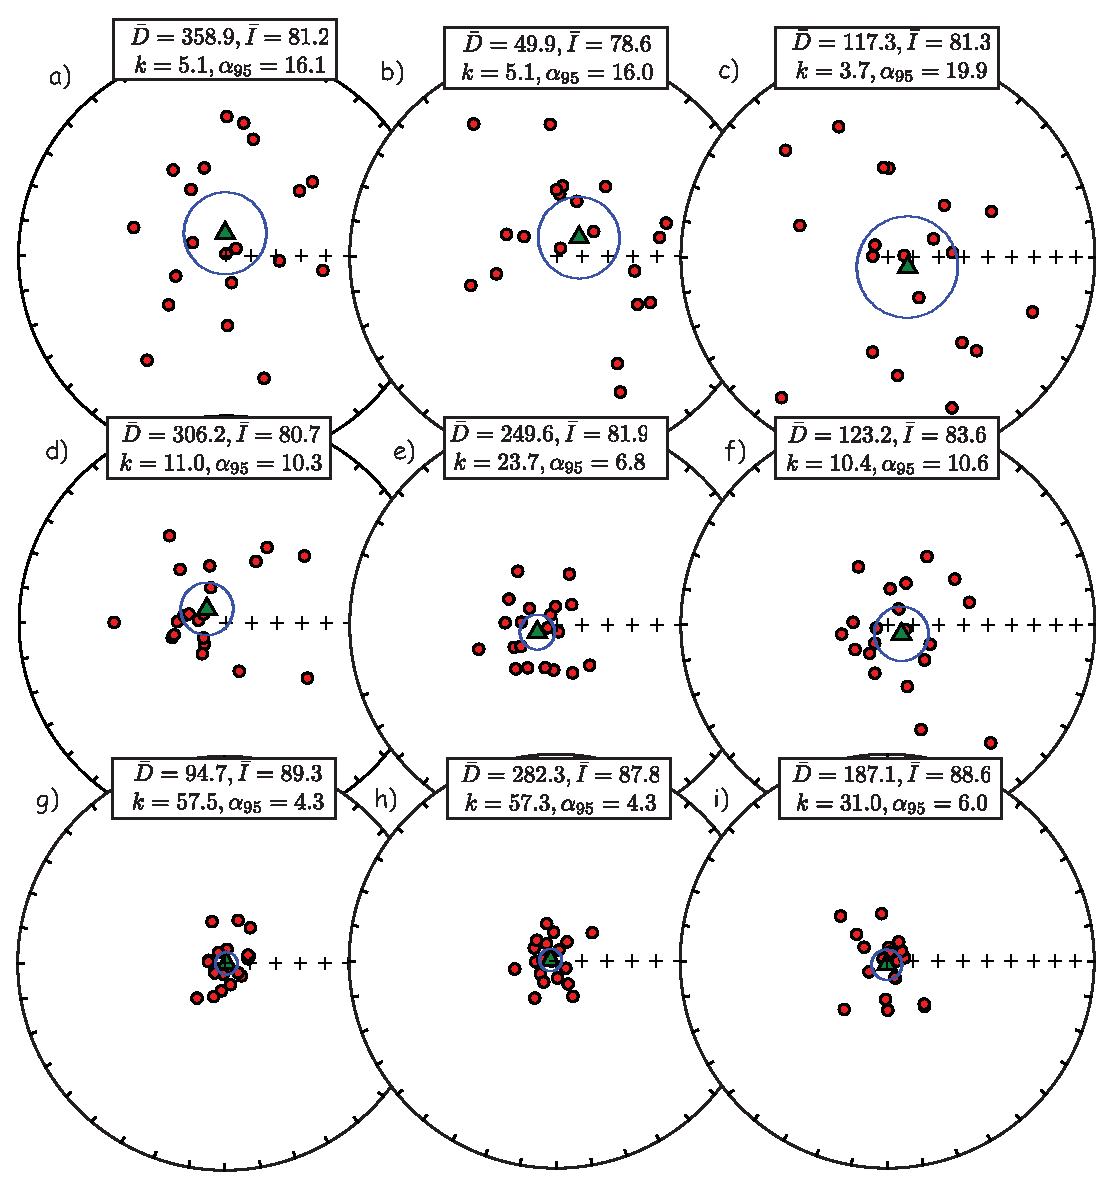
\includegraphics[width= 12 cm]{EPSfiles/fisher.eps}
\caption {Hypothetical data sets drawn from Fisher distributions with vertical true directions with $\kappa $ = 5  (a-c), $\kappa $ = 10 (d-f),  $\kappa$ = 50 (g-i).  Estimated $\bar D, \bar I, \kappa, \alpha_{95}$ shown in insets.  
}
\label{fig:fisher}
\end{figure}


In order to calculate mean directions with confidence limits, paleomagnetists
rely heavily on the special statistics 
known as 
\index{Fisher!statistics}
{\it Fisher statistics}
\index{Fisher, R.A.}
(Fisher, 1953), \nocite{fisher53}
which were developed for assessing dispersion of unit vectors on a sphere. It is applicable to directional data that are dispersed in a symmetric manner about the true direction.  We show some examples of such data in Figure~\ref{fig:fisher} with varying amounts of scatter from highly scattered in the top row to rather concentrated in the bottom row.  All the data sets were drawn from a Fisher distribution with a  vertical true direction.  

  In most instances, paleomagnetists assume a
Fisher distribution for their data because the statistical treatment allows
calculation of confidence intervals, comparison of mean directions,
 comparison of scatter, etc.
 The average inclination, calculated as the arithmetic mean of the inclinations,
will  never be vertical unless all the inclinations are vertical.  
In the following, we will demonstrate the proper way to
calculate mean directions and confidence regions for directional data
that are distributed in the manner shown in Figure~\ref{fig:fisher}.  We
will also briefly describe several useful statistical tests that are popular in the
paleomagnetic literature.     

 


\subsection {Estimation of Fisher statistics}
\label{sect:fisher}


\index{Fisher, R.A.}
R. A. Fisher  developed a probability density function applicable to many paleomagnetic directional data sets, known as the
\index{Fisher!distribution}
\index{distributions!Fisher}
 Fisher distribution  (Fisher, 1953).  In Fisher statistics each direction is given unit weight and is represented
by a point on a sphere of unit radius. The Fisher distribution function $P_{dA}(\alpha)$ gives the probability per
unit angular area of finding a direction within an angular area, $dA$, centered at an angle $\alpha$ from the true mean.
The angular area, $dA$, is expressed in steredians, with the total angular area of a sphere being $4\pi$ steredians.
Directions are distributed according to the 
\index{Fisher!probability density function}
the Fisher probability density,  given by:

\begin{equation} 
{P_{dA}(\alpha)} = {\kappa \over 4\pi \sinh \kappa} \exp (\kappa \cos \alpha), 
\label{eq:fishdis}
\end{equation}

\noindent where  $\alpha $ is the angle between the unit vector and
the true direction and $\kappa $ is a {\it precision parameter} such that as $\kappa
\to \infty$, dispersion goes to zero. 



We can see in Figure~\ref{fig:P}a the probability of finding a direction  within an angular area $dA$ centered $\alpha$ degrees away from the true mean  for different values of $\kappa$.  $\kappa$ is a measure of the concentration of the distribution about the true mean direction. The larger the value of $\kappa$, the more concentrated the direction;   $\kappa$ is 0 for a distribution of directions that is uniform over the sphere and approaches $\infty$ for directions concentrated at a point.   

\begin{figure}[htb]
%\epsfxsize 14cm
%\centering \epsffile{EPSfiles/P.eps}
\centering  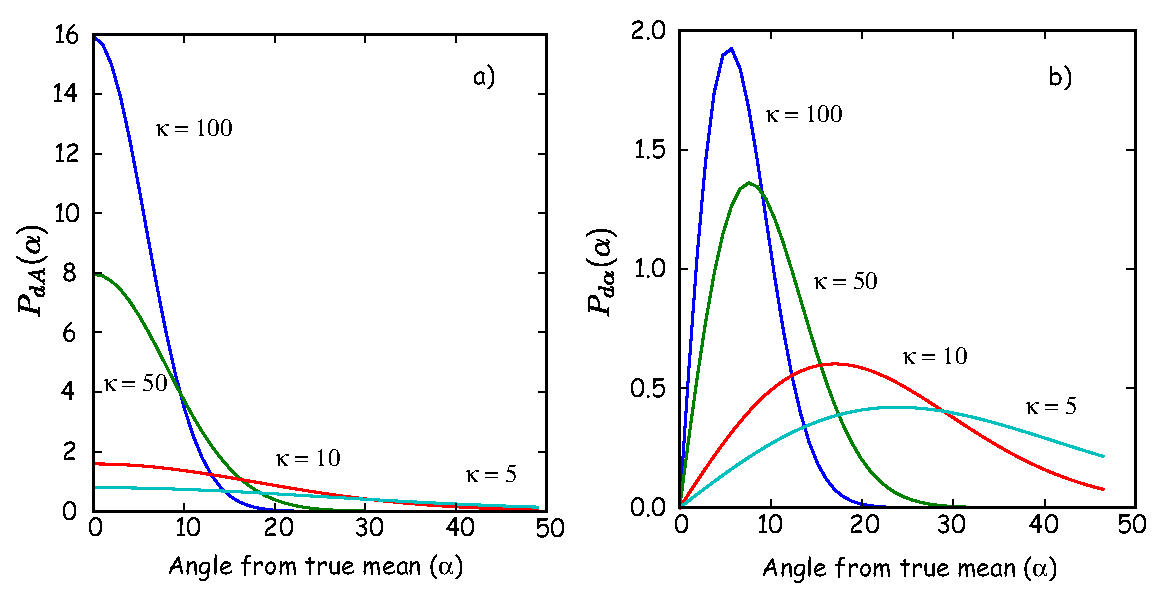
\includegraphics[width= 14 cm]{EPSfiles/P.eps}
\caption{a) Probability of finding a direction within an angular area, $dA$ centered at an angle $\alpha$ from the true mean.   b) Probability of finding a direction at angle $\alpha$ away from the true mean direction.}
\label{fig:P}
\end{figure}

If $\phi$ is taken as the azimuthal angle about the true mean direction, the probability of a direction within an
angular area, $dA$, can be expressed as

$$
P_{dA}(\alpha) dA= P_{dA}(\alpha)\sin (\alpha) d\alpha d\phi.
$$

\noindent The $\sin \alpha$ term arises because the area of a band of width $d\alpha$ varies as $\sin \alpha$.  It should be understood that the 
\index{distributions!Fisher}
Fisher distribution is normalized so that 

\begin{equation}
\int_{\phi=0}^{2\pi} \int_{\alpha=0}^{\pi}  P_{dA} (\alpha) \sin (\alpha) d\alpha d\phi = 1.
\label{eq:fishnorm}
\end{equation}

\noindent Equation~\ref{eq:fishnorm} simply indicates that the probability of finding a direction somewhere on the unit sphere must be unity.  The probability $P_{d\alpha}$ of finding a direction in a band of width $d\alpha$ between $\alpha$ and $\alpha+d\alpha$ is given by:

$$
P_{d\alpha} (\alpha) = \int_{\phi=0}^{2\pi} P_{dA} (\alpha)dA = 2\pi P_{dA} (\alpha) \sin (\alpha) d\alpha
$$
 
\begin{equation}
\hskip 1em = {P_{dA}(\alpha)}  \sin \alpha = {\kappa \over 2\pi \sinh \kappa} \exp (\kappa \cos \alpha) \sin
\alpha.
\label{eq:fishpde}
\end{equation}

\noindent This probability (for $\kappa = 5, 10, 50, 100$) is shown in Figure~\ref{fig:P}b where the effect of the $\sin \alpha$ term is apparent.  
Equation~\ref{eq:fishdis} for the 
\index{Fisher!distribution}
Fisher distribution function
suggests that declinations are symmetrically  distributed about the mean.  In
``data'' coordinates, this means that the declinations are uniformly distributed from 0
$\rightarrow$ 360$^{\circ}$.  Furthermore, the probability $P_{\alpha}$ of finding a
direction of $\alpha$ away from the mean decays exponentially.



Because the intensity of the magnetization has little to do with the
validity of the measurement (except for very weak magnetizations), it
is customary to assign
unit length to all directions.
\index{Fisher!mean}%
  The mean direction is calculated by first
converting the individual moment directions ($m_i$) (see Figure~\ref{fig:vecsum}), which may be  expressed as declination and inclination ($D_i,I_i$),  
 to cartesian coordinates ($x_1,x_2,x_3$) by the methods given in Chapter 2.  Following the logic for vector addition explained in Appendix~\ref{app:vectors}, the length of the  vector sum, or 
\index{Fisher!resultant vector}%
resultant vector  $R$, is given by:

\begin{equation} 
{R^2} = (\sum_{i} x_{1i})^2 + (\sum_i x_{2i})^2 + (\sum_i x_{3i})^2,
\label{eq:R}
\end{equation}


\noindent
The relationship of $R$ to the $N$ individual unit vectors is shown in Figure~\ref{fig:vecsum}. $ R$ is always $<N$ and approaches
$N $ only when the vectors are tightly clustered. The mean direction components  are given by:

\begin{equation} 
\bar x_1 = {1\over R} (\sum_i x_{1i}) ; \hskip 1em \bar x_2 = {1\over R} (\sum_i x_{2i}); \hskip 1em 
 \bar x_3 = {1\over R} (\sum_i x_{3i}).
\label{eq:xbar} \end{equation}

\noindent
These cartesian coordinates 
can, of course, be converted back to geomagnetic elements ($\bar D,
\bar I$) by the familiar method described in  Chapter 2.


\begin{figure}[htb]
%\epsfxsize 10cm
%\centering \epsffile{EPSfiles/vecsum.eps}
\centering  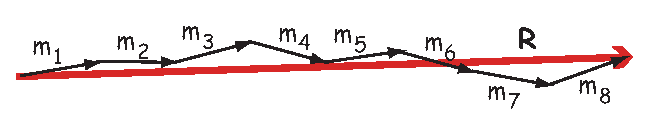
\includegraphics[width= 10 cm]{EPSfiles/vecsum.eps}
\caption{Vector addition of eight unit vectors ($m_i$) to yield resultant vector $R$.  [Figure redrawn from Butler, 1992.]  }
\label{fig:vecsum}
\end{figure}  


\index{Fisher!precision parameter}%
Having calculated the mean direction, the next objective is to determine a statistic that can provide a measure
of the dispersion of the population of directions from which the sample data set was drawn. One
measure of the dispersion of a population of directions is the precision parameter, $\kappa$. From a finite sample
set of directions, $\kappa$ is unknown, but a best estimate of $\kappa$  can be calculated by

\begin{equation}
\kappa \simeq k
={{N-1}\over {N-R}},
\label{eq:k}
\end{equation}

\noindent  where $N$ is the number of data points. 
Using this
estimate of $\kappa $, we estimate the circle of 95\% confidence ($p=0.05$) about the
mean, $\alpha_{95}$, by:
\index{Fisher!circle of 95\% confidence}%

\begin{equation}
\alpha_{95}=\hbox {cos}^{-1}\bigl[1 - {{N-R}\over {R}}\bigl[
\bigl({1\over {p}}\bigr)^{1\over
{(N-1)}}-1\bigr]\bigr].
\label{eq:a95}
\end{equation}
In the classic paleomagnetic literature, $\alpha_{95}$ was further approximated
by:
$$
\alpha_{95}' \simeq {{140}\over {\sqrt{k N}}} ,
$$
\noindent which is  reliable for $k$ larger than
about 25 (see 
\index{Tauxe, L.}
 Tauxe et al., 1991).\nocite{tauxe91} 
By direct analogy with Gaussian statistics (Equation~\ref{eq:sigma}), the angular variance of a sample set of directions is:

\begin{equation}
S^2 = { 1 \over {N-1}} \sum_{i=1} ^N \Delta_i^2,
\label{eq:S}
\end{equation}

\noindent where $\Delta_i$ is the angle between the $i^{th}$ direction and the calculated mean direction.  The estimated
\index{Fisher!circular standard deviation}
 circular (or angular) standard deviation is $S$, which can be approximated by: 


\begin{equation}
CSD \simeq {{81}\over {\sqrt{k}}},
\label{eq:csd}
\end{equation}
\noindent which is the circle containing $\sim$63\% of the data.

Some practitioners use the statistic $\delta$ given by:

\begin{equation}
\delta = \cos^{-1} \bigl( {R\over N} \bigr),
\label{eq:del}
\end{equation}
\noindent because of its ease of calculation and the intuitive appeal (e.g., Figure~\ref{fig:vecsum}) that $\delta$ decreases as $R$ approaches $N$.  In practice,  when $N>\sim 10-20$,  CSD and $\delta$ are close to equal.  


When we calculate the mean direction, a dispersion estimate, and a confidence limit, we are supposing
that the observed data came from random sampling of a population of directions accurately
described by the 
\index{Fisher!distribution}
Fisher distribution. But we do not know the true mean of that Fisherian population,
nor do we know its precision parameter $\kappa$. We can only estimate these unknown parameters. The
calculated mean direction of the directional data set is the best estimate of the true mean direction,
while $k$ is the best estimate of $\kappa$. The confidence limit $ \alpha_{95}$ is a measure of the precision with which the
true mean direction has been estimated. One is 95\% certain that the unknown true mean direction lies
within $\alpha_{95}$ of the calculated mean. The obvious corollary is that there is a 5\% chance that the true
mean lies more than $\alpha_{95}$ from the calculated mean.


%\clearpage
\subsection{Some illustrations}

Having buried the reader in mathematical formulations, we present the following illustrations to develop some
intuitive appreciation for the statistical quantities. One essential concept is the distinction between statistical
quantities calculated from a directional data set and the unknown parameters of the sampled population.


Consider the various sets of directions plotted as equal area projections (see Chapter  2) in
Figure~\ref{fig:fisher}.  These are all synthetic data sets drawn from 
\index{Fisher!distribution}
Fisher distributions  with means of a single, vertical direction.     Each  of the three diagrams in a row is a a  replicate sample from the same distribution. The top row were all drawn from a distribution with $\kappa= 5$, the middle with $\kappa=10$ and the bottom row with $\kappa=50$.     For each synthetic data set, we estimated $\bar D, \bar I, \kappa$ and $\alpha_{95}$ (shown as insets to the equal area diagrams).  

There are several important observations to be taken from these  examples. Note that the calculated mean
direction is never exactly the true mean direction ($I $ = +90$^{\circ}$). The calculated mean inclination $\bar I$ varies from
78.6$^{\circ}$  to 89.3$^{\circ}$, and the  mean declinations fall  within all quadrants of the equal-area projection.   The calculated mean direction thus randomly dances about the true mean direction
and deviates from the true mean by between 0.7$^{\circ}$ and 11.4$^{\circ}$.
The calculated $k$  statistic varies considerably among replicate samples as well.   The variation of $k$ and differences in angular
variance of the data sets with the same underlying distribution are simply due to the vagaries of random sampling. 

The confidence limit $\alpha_{95}$  varies from 19.9$^{\circ}$ to 4.3$^{\circ}$ and is shown by the circle surrounding the
calculated mean direction (shown as a triangle). For these directional data sets, only one (Figure~\ref{fig:fisher}e)  has a calculated mean that is more than
$\alpha_{95}$ from the true mean. However, if 100 such synthetic data sets had been analyzed, on average five  would have a calculated mean direction removed from the true mean direction by more than the calculated
confidence limit $\alpha_{95}$. That is, the true mean direction would lie outside the circle of 95\% confidence, on
average, in 5\% of the cases.

It is also important to appreciate which statistical quantities are fundamentally dependent upon the
number of observations N. Neither the $k$ value (Equation~\ref{eq:k}) nor the estimated angular deviation CSD 
(Equation~\ref{eq:csd}) is fundamentally dependent upon $N$. These statistical quantities are estimates of
the intrinsic dispersion of directions in the Fisherian population from which the data set was sampled. Because
that dispersion is not affected by the number of times the population is sampled, the calculated
statistics estimating that dispersion should not depend fundamentally on the number of observations $N$.
However, the confidence limit $\alpha_{95}$  should depend on $N$; the more individual measurements there are in
our sample, the greater must be the precision (and accuracy) in estimating the true mean direction. This increased precision
should be reflected by a decrease in $\alpha_{95}$  with increasing $N$. Indeed Equation~\ref{eq:a95} indicates that $\alpha_{95}$ 
depends approximately on $1/ \sqrt{N}$ .

Figure~\ref{fig:a95-csd} illustrates these dependencies of calculated statistics on number of directions in a data set.   This diagram was constructed as follows:

\begin{enumerate}
\item We drew a synthetic data set of $N=30$ from a Fisher distribution with a $\kappa$ of 29.2 (equivalent to a circular standard deviation $S$ of 15$^{\circ}$). 
\item  Starting with the first four directions in the synthetic data set, a subset of $N$ = 4 was used to
calculate $k$,  CSD and $\delta$ using Equations~\ref{eq:k}, ~\ref{eq:csd}, and ~\ref{eq:del} respectively.   In
addition, $\alpha_{95}$ (using Equation~\ref{eq:a95}) was calculated. Resulting values of CSD, $\delta$ and $\alpha_{95}$ are shown in Figure~\ref{fig:a95-csd} as a function of $N$.  
\item For each succeeding value of $N $ in Figure~\ref{fig:a95-csd}, the next direction from the $N$ = 30 synthetic data set
was added to the previous subset of directions, continuing until the full $N$ = 30 synthetic data set was
used.
\end{enumerate}

The effects of increasing $N$ are readily apparent in Figure~\ref{fig:a95-csd} in which we show  a comparison of the two estimates of $S$, CSD and $\delta$.    
Although not fundamentally dependent
upon $N$, in practice the estimated angular standard deviation, CSD, deviates from  $S$ for values of $N < 15$, only approaching the correct value when  $N \ge 15$. As expected, the calculated confidence limit $\alpha_{95}$ decreases
approximately as $1 / \sqrt{N}$ , showing a dramatic decrease in the range $4 < N < 10 $ and more gradual decrease
for $N > 10$.   




\begin{figure}[htb]
%\epsfxsize 10cm
%\centering \epsffile{EPSfiles/a95-csd.eps }
\centering  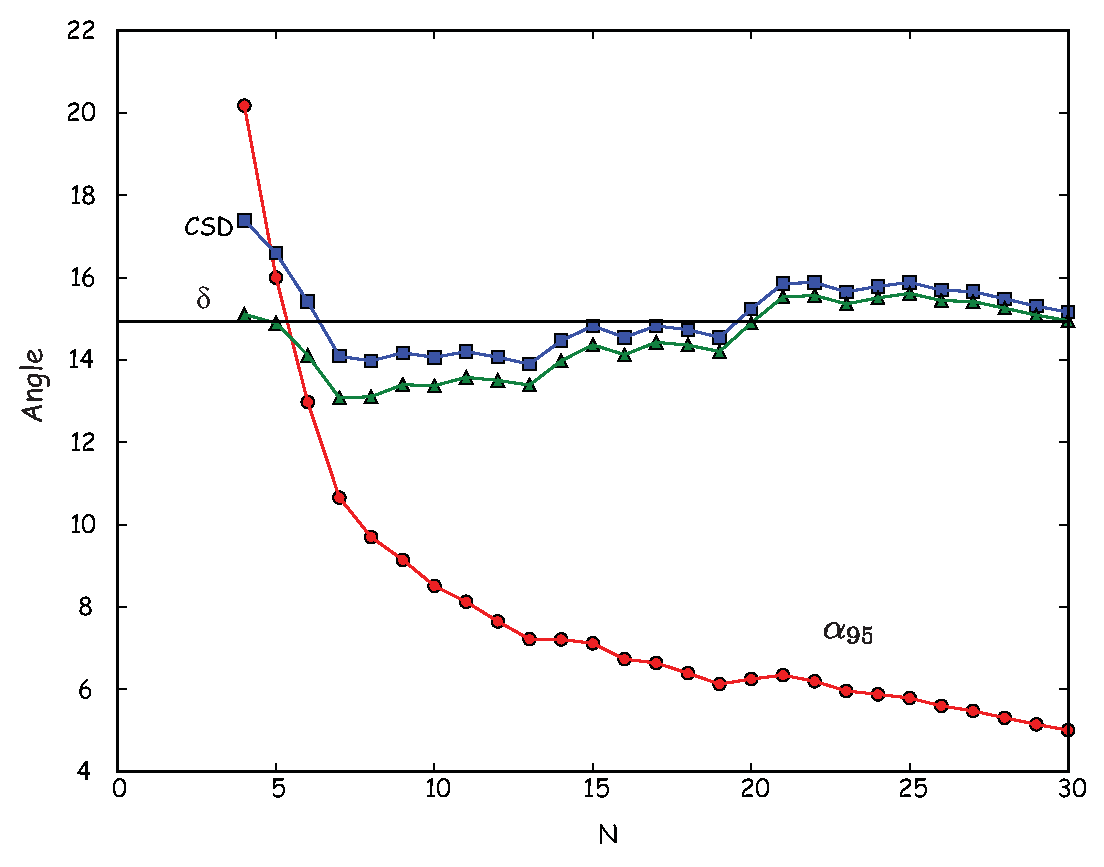
\includegraphics[width= 10 cm]{EPSfiles/a95-csd.eps}
\caption { Dependence of estimated angular
standard deviation, CSD and $\delta$, and confidence
limit, $\alpha_{95}$, on the number of directions
in a data set. An increasing number
of directions were selected from a
Fisherian sample of directions with
angular standard deviation $S$ = 15$^{\circ}$
($\kappa$ = 29.2),  shown by the horizontal line.
}
\label{fig:a95-csd}
\end{figure}




If directions are converted to VGPs as outlined in Chapter 2,  the
transformation distorts a rotationally symmetric set of data
into an elliptical distribution.  The associated $\alpha_{95}$  may  no
longer be appropriate.  
\index{Cox, A.}
\index{Doell, R.R.} 
Cox and Doell (1960) \nocite{cox60}  suggested the following for 95\% confidence regions in 
VGPs.  Ironically, it is more likely that the VGPs are spherically symmetric implying that most sets of directions are not!

\begin{equation}
dm = {\alpha_{95}}{\cos \lambda \over {\cos \bar I}}, \hskip 1em dp = {1\over 2}{\alpha_{95}}{(1 + 3 \sin^2 \lambda)},
\label{eq:dpdm}
\end{equation}

\noindent where $dm$ is the semi-axis parallel to  the meridians 
(lines of longitude), $dp$is the semi-axis parallel to the parallesl
(lines of latitude), and $\lambda$ is the site paleolatitude.


\section{Significance Tests}

The Fisher distribution allows us to ask a number of questions about paleomagnetic data sets, such as:

\begin{enumerate}
\item Is a given set of directions random?  This is the question that we ask when we perform a conglomerate test (Chapter  9).

\item Is one data set better grouped than another as in the fold test from Chapter 9. 

\item Is the mean direction of a given (Fisherian) data set 
different from some known direction?  This question comes up when we compare a given data set with, for example, the directions of the present or GAD field.

\item Are two (Fisherian) data sets different from each other?  For example, are the normal directions and the antipodes of the reversed directions the same for a given data set?

\item If a given site has some samples that allow only the calculation of a
best-fit plane and not a directed line, what is the site mean direction
that 
combines the best-fit lines and planes (see Chapter  9)?   

\end{enumerate}

In the following discussion, we will briefly summarize ways of addressing these issues
using Fisher techniques.    There are two fundamental principles of statistical significance tests that are important to the proper
interpretation:

\begin{enumerate}
\item
 Tests are generally made by comparing an observed sample with a {\it null hypothesis}. For example, in
comparing two mean paleomagnetic directions, the null hypothesis is that the two mean directions
are separate samples from the same population of directions. (This is the same as saying that the
samples were not, in fact, drawn from different populations with distinct true mean directions.) Significance
tests do not disprove a null hypothesis but only show that observed differences between the
sample and the null hypothesis are unlikely to have occurred because of sampling limitations. In other
words, there is probably a real difference between the sample and the null hypothesis, indicating
that the null hypothesis is probably incorrect.
\item  Any significance test must be applied by using a level of significance. This is the probability level at
which the differences between a set of observations and the null hypothesis may have occurred by
chance. A commonly used significance level is 5\%. In Gaussian statistics, when testing an observed
sample mean against a hypothetical population mean $\mu$ (the null hypothesis), there is only a
5\% chance that $x$  is more than 2$\sigma_m$ from the mean, $\mu$, of the sample. If $\bar x$ differs from $\mu$ by more
than 2$s$, $\bar x$ is said to be ``statistically different from $\mu$ at the 5\% level of significance,''  using proper
statistical terminology. However, the corollary of the actual significance test is often what is reported
by statements such as ``$\bar x$  is distinct from $\mu$ at the 95\% confidence level.''  The context usually makes
the intended meaning clear, but be careful to practice safe statistics.
\end{enumerate}

An important sidelight to this discussion of level of significance is that too much emphasis is often put on
the 5\% level of significance as a magic number. Remember that we are often performing significance tests
on data sets with a small number of observations. Failure of a significance test at the 5\% level of significance
means only that the observed differences between sample and null hypothesis cannot be shown to
have a probability of chance occurrence that is $>$ 5\%. This does not mean that the observed differences are
unimportant. Indeed the observed differences might be significant at a marginally higher level of significance
(for instance, 10\%) and might be important to the objective of the paleomagnetic investigation.

Significance tests for use in paleomagnetism were developed in the 1950s by
\index{Watson, G.S.}
\index{Irving, E.A.}
G.S.  Watson and E.A. Irving. These versions of the significance tests are fairly simple, and an intuitive appreciation
of the tests can be developed through a few examples. Because of their simplicity and intuitive appeal,
we investigate these ``traditional'' significance tests in the development below. However, many of these tests
have been updated using advances in statistical
sampling theory. These will be discussed in Chapter 12.  While they are technically superior to the traditional significance tests,  they are more complex and less intuitive than
the traditional tests.


\subsection {Watson's test for randomness}
\label{sect:Ro}


\index{statistical tests!randomness}%
\index{Watson, G.S.}
Watson (1956) \nocite{watson56}
 demonstrated how to test a given directional
data set for randomness.  His test
relies on the calculation of $R$ given by Equation~\ref{eq:R}.  Because $R$ is the
length of the resultant vector, randomly directed vectors will have small values of $R$,
while, for less scattered directions, $R$ will approach $N$.  
Watson (1956) defined a parameter $R_o$ that can be used for testing 
the randomness of a given data set.  If the value of  $R$  
exceeds $R_o$, the null hypothesis of total randomness can be rejected at a
specified level of confidence.  If $R$
is less than $R_o$, randomness cannot be rejected. 
Watson calculated the value of $R_o$ for a range of $N$ for the 95\% and 99\%  confidence levels.  Watson  (1956) also showed how to estimate $R_o$ by:
\begin{equation}
R_o=\sqrt{ 7.815 \cdot N/3}.
\label{eq:Ro}
\end{equation}
\noindent The estimation works well for $N>10$, but
is somewhat biased for smaller data sets.  The critical
values of $R$ for $5<N< 20$ from
\index{Watson, G.S.}%
 Watson  (1956) are listed
for convenience in Table~\ref{tab:Ro}.  




The test for randomness is particularly useful for determining if, for
example, the directions from a given site are randomly oriented
(the data for the  site should therefore be thrown out).  Also, 
one can determine  if directions from
\index{paleomagnetic tests!conglomerate}%
the conglomerate test are random or not (see Chapter 9).  


\subsection{Comparison of precision } 

In the 
\index{paleomagnetic tests!fold}
fold test (or bedding-tilt test), one examines the clustering of directions before and after performing
structural corrections. If the clustering improves on structural correction, the conclusion is that the ChRM
was acquired prior to folding and therefore ``passes the fold test''. The appropriate significance test determines
whether the improvement in clustering is statistically significant.  Here we will discuss a very quick, back of the envelope test for this proposed by 
\index{McElhinny, M.W.}
McElhinny (1964).     \nocite{mcelhinny64}This form of the fold test is not used much anymore (see 
\index{McFadden, P.L.}
\index{Jones, D.L.}
McFadden and Jones, 1981), \nocite{mcfadden81} but serves as a quick and intuitively straight-forward introduction to the subject.  

Consider two directional data sets, one with $N_1$ directions and $k_1$, and one with $N_2$ directions and $k_2$. If
we assume (null hypothesis) that these two data sets are samples of populations with the same $k$, the ratio
$k_1 / k_2$ is expected to vary because of sampling errors according to

\begin{equation}
{ k_1 \over {k_2}} = {  { \hbox{var} [2(N_2 -1)]} \over { \hbox{var} [ 2(N_1 -1)]}},
\label{eq:k1-k2}
\end{equation}

\noindent where $\hbox{var} [2(N_2 -1)]$ and $\hbox{var} [2(N_1 -1)]$ are variances with $2(N_2-1)$ and $2(N_1-1)$ degrees of freedom.  This ratio should follow the F-distribution if the assumption of common $\kappa$  is correct. Fundamentally, one expects
this ratio to be near 1.0 if the two samples were, in fact, selections from populations with common $\kappa$. The
F-distribution tables indicate how far removed from 1.0 the ratio may be before the deviation is significant at
a chosen probability level. If the observed ratio in Equation~\ref{eq:k1-k2}  is far removed from 1.0, then it is highly
unlikely that the two data sets are samples of populations with the same $\kappa$. In that case, the conclusion is
that the difference in the $\kappa$ values is significant and the two data sets were most likely sampled from populations
with different $\kappa$.

As applied to the fold test, one examines the ratio of $k$ after tectonic correction ($k_a$) to $k $ before
tectonic correction ($k_b$). The significance test for comparison of precisions determines whether $k_a / k_b$
is significantly removed from 1.0. If $k_a / k_b$ exceeds the value of the F-distribution for the 5\% significance
level, there is less than a 5\% chance that the observed increase in k resulting from the tectonic
correction is due only to sampling errors. There is 95\% probability that the increase in $k$ is meaningful
and the data set after tectonic correction is a sample of a population with $k$ larger than the population
sampled before tectonic correction. Such a result constitutes a ``statistically significant passage of the
fold test.''   









\begin{figure}[h!tb]
%\epsfxsize 14cm 
%\centering \epsffile{EPSfiles/twosets.eps}
\centering  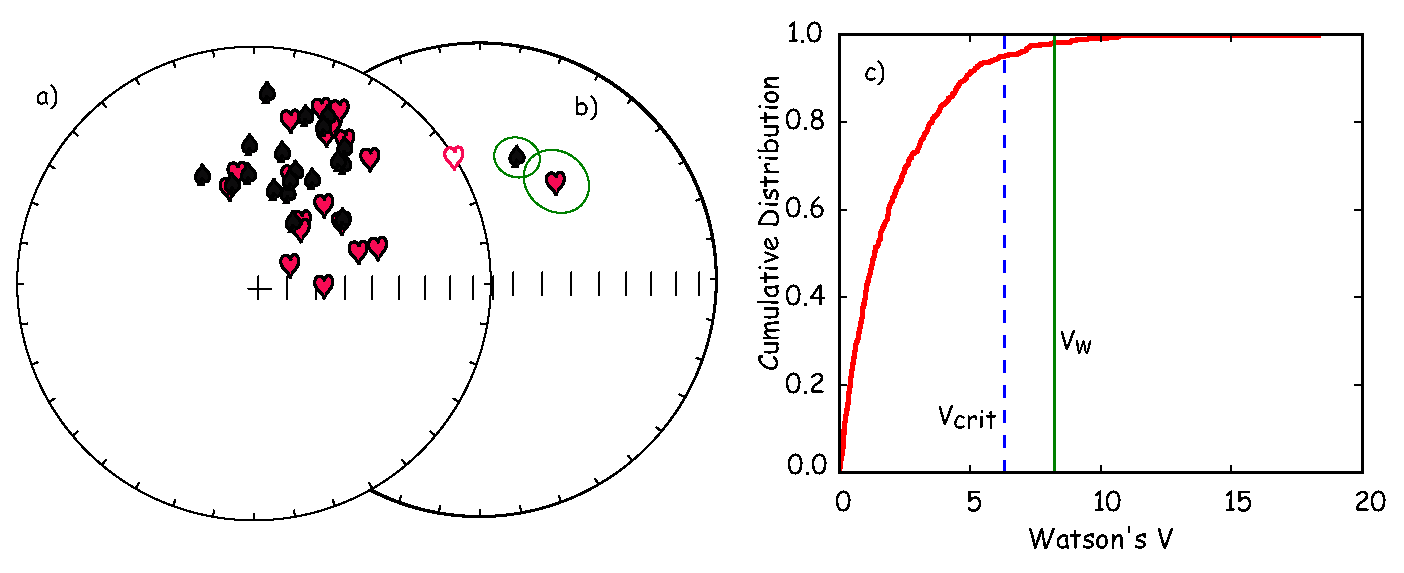
\includegraphics[width= 14 cm]{EPSfiles/twosets.eps}
\caption{a) Equal area projections of declinations and inclinations of  two hypothetical data sets.
b) Fisher means  and circles of confidence from the data sets in a). c) Distribution of $V_w$ for simulated Fisher distributions with the same $N$ and $\kappa$ as the two shown in a).  The dashed line is the upper bound for  the smallest 95\% of the $V_w$s calculated for the simulations ($V_{crit}$).  The solid vertical line is the $V_w$ calculated for the two data sets.  According to this test, the two data sets do not have a common mean, despite their overlapping confidence ellipses.}
\label{fig:twosets}
\end{figure}

\subsection {Comparing known and estimated directions}

The calculation of confidence regions for paleomagnetic
data is largely motivated by a need to compare  estimated directions with
either a known direction (for example, the present field) or another estimated
direction (for example, that expected for a particular paleopole, the present field or a GAD field). 
Comparison of a paleomagnetic data set with a given direction is  
straight-forward using Fisher statistics. 
 If the known test direction lies outside the
confidence interval computed for the estimated direction, then the estimated and
known directions are different at the specified confidence level. 

\begin{figure}[h!tb]
%\epsfxsize 14cm
%\centering \epsffile {EPSfiles/lnp.eps}
\centering  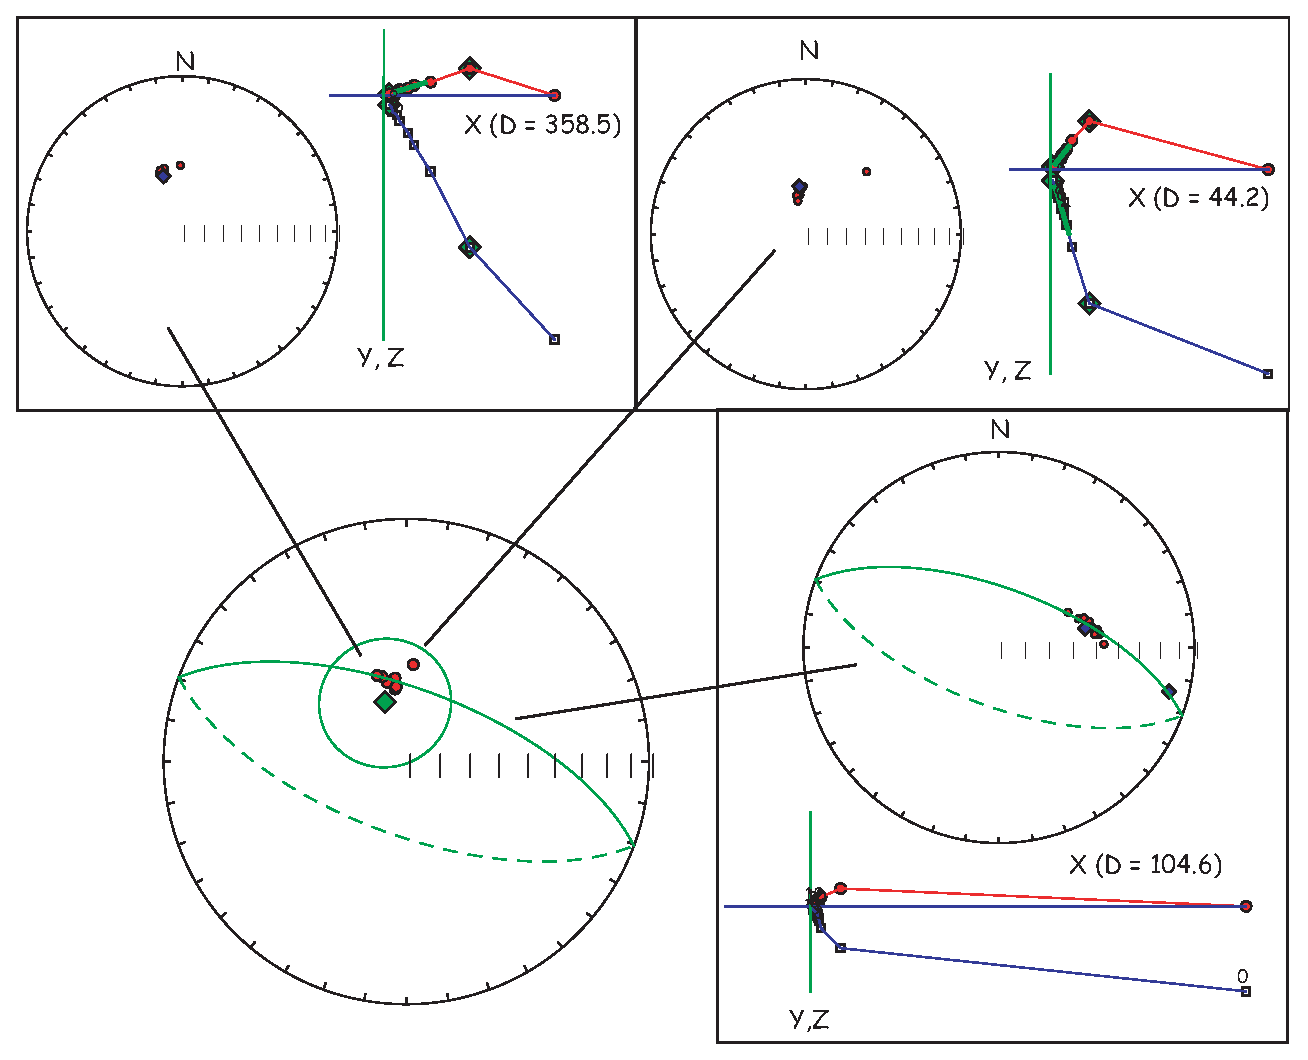
\includegraphics[width= 14 cm]{EPSfiles/lnp.eps}
\caption{
Examples of demagnetization data from a site whose mean is partially
constrained by  a great circle. 
 The best-fit great
circle and six directed lines allow a mean (diamond) and 
associated $\alpha_{95}$ to
be calculated using the method of 
\index{McFadden, P.L.}%
McFadden and 
\index{McElhinny, M.W.}%
McElhinny (1988).   Demagnetization data for two of the directed lines are shown at the top of the diagram while those for the great circle are shown at the bottom.  [Data from Tauxe et al., 2003.]  
}
\label{fig:lnp}
\end{figure} \nocite{tauxe03b}

\subsection {Comparing two estimated directions}

The case in which we are comparing  two Fisher distributions  can also be
relatively straight forward. 
If the two confidence circles do not overlap, the two directions are 
different at the specified (or more stringent) level of certainty.  When one confidence region includes
the mean of the other set of directions, the difference in directions is not
significant.  

The situtation becomes a little more tricky when the data sets are as shown in Figure~\ref{fig:twosets}a.  The Fisher statistics for the two data sets are:

\vskip 6pt
\begin{center}
\begin{tabular}{cccccccc}
\hline
$i$ & symbol& $\bar D$ & $\bar I$ & $N$ & $R$ & $k$&$\alpha_{95}$\\
\hline 
1&spades&  38.0&   45.7  &   20  & 18.0818    &  9.9   &10.9\\
2 & hearts&   16.9   &45.2   &  20 &  19.0899&     20.9  &  7.3\\
\hline
\end{tabular}
\end{center}

As shown in the equal area projection in Figure~\ref{fig:twosets}b, the two $\alpha_{95}$s overlap, but neither includes
the mean of the other. This sort of
``grey zone'' case  has been  addressed by many workers. 


The most common  way of testing the significance of two sets of directions is a simple 
\index{statistical tests!Watson's $F$}
$F$ test, proposed by 
\index{Watson, G.S.}
Watson (1956b).  \nocite{watson56b}
Consider two directional data sets: one has $N_1$ directions (described by unit vectors) yielding a resultant
vector of length $R_1$; the other has $N_2$ directions yielding resultant $R_2$. The statistic

\begin{equation}
F = {(N - 2)} {{(R_1 + R_2 - R)}  \over {(N - R_1 - R_2 )} },
\label{eq:twoF}
\end{equation}

\noindent must be determined, where
$N = N_1 + N_2$
and $R$ is the resultant of all $N$ individual directions. This $F$ statistic is compared with tabulated values for 2
and 2($N$-2) degrees of freedom. If the observed $F$ statistic exceeds the tabulated value at the chosen
significance level, then these two mean directions are different at that level of significance.

The tabulated F-distribution indicates how different two sample mean directions can be (at a chosen
probability level) because of sampling errors. If the calculated mean directions are very different but the
individual directional data sets are well grouped, intuition tells us that these mean directions are distinct.
The mathematics described above should confirm this intuitive result. With two well-grouped directional
data sets with very different means, $ (R_1 + R_2) >> R, R_1 \rightarrow N_1$, and $R_2 \rightarrow N_2$, so that ($R_1 + R_2) \rightarrow N$. With these conditions, the F statistic given by Equation~\ref{eq:twoF}  will be large and
will easily exceed the tabulated value. So this simple intuitive examination of Equation~\ref{eq:twoF}  yields a
sensible result.


\begin{figure}[htb]
%\epsfxsize 7.5cm
%\centering \epsffile{EPSfiles/incfish.eps}
\centering  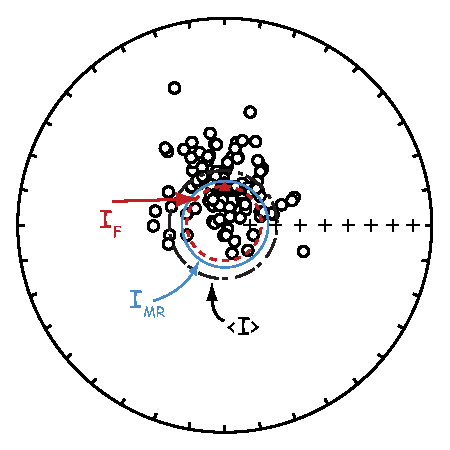
\includegraphics[width= 7.5 cm]{EPSfiles/incfish.eps}
\caption{Directions drawn from a Fisher distribution with a near vertical true
mean direction.  The Fisher mean direction from the sample is shown by the
triangle.  The Gaussian average inclination ($<I>= 70^{\circ}$) is shallower than the
Fisher mean $I_F = 75^{\circ}$. The estimated inclination using the maximum likelihood estimate of McFadden and Reid (1982) ($I_{MF}=73^{\circ}$ is closer to the Fisher mean than the Gaussian average).}
\label{fig:incfish}
\end{figure} \nocite{mcfadden82}



  An alternative, and in many ways superior,  statistic ($V_w$) was proposed by 
  \index{Watson, G.S.}
  Watson
(1983; see Appendix~\ref{app:watsonsV} for details).   \nocite{watson83}
\index{statistical tests!Watson's $V_w$}
$V_w$ was posed as a test statistic that increases with increasing difference between the mean
directions of the two data sets.  Thus, the null hypothesis that two data sets have a common mean
direction can be rejected if $V_w$ exceeds some critical value which can be determined through what is called
{\it Monte Carlo simulation}.  The technique gets its name from a famous gambling locale because we use randomly drawn samples (``cards'') from specified  distributions (``decks'')  to 
see what can be expected from chance.  What we want to know is  the probability that two data sets (hands of cards?) drawn from the same underlying distribution would have a given $V_w$ statistic just from chance.  

We proceed as follows:

\begin{enumerate}
\item Calculate the $V_w$ statistic for the data sets.  [The  $V_w$
for the two data sets shown in  Figure~\ref{fig:twosets}a is  8.5.]

\item In
order to determine the critical value for $V_w$, we draw two Fisher distributed data sets with
dispersions of $k_1$ and $k_2$ and $N_1, N_2$, but having  a common true direction.  

\item We then calculate
$V_w$ for these simulated data sets.

\item   Repeat  the simulation some large number of  times (say 1000).   This defines the distribution of $V_w$s that you would get from chance by ``sampling''   distributions with the same direction.  

\item Sort the $V_w$s in order of increasing size.  The critical value of $V_w$ at the 95\% level of confidence is the 950$^{th}$ simulated $V_w$.  
\end{enumerate}

 The $V_w$s simulated for two distributions with the same $\kappa$ and $N$  as our  example data sets but drawn from distributions with the same mean are
plotted as a cumulative distribution function in Figure~\ref{fig:twosets}c with the bound containing the lowermost 95\%  of the  simulations shown
as a dashed line at 6.2.  The value of 8.5, calculated for the data set  is shown as a heavy vertical line 
and is clearly larger than  95\% of the simulated populations. This simulation
therefore supports the suggestion  that the two data sets do not have a common mean at the 95\% level of confidence.    

This test can be applied to the two polarities in a given data collection to see if they are antipodal.  In this case, one would take the antipodes of one of the data sets before calculating $V_w$.  
Such a  test would be  a Fisherian form of the {\it reversals test}.





\subsection {Combining directions and great circles}

 Consider the demagnetization data  shown in
Figure~\ref{fig:lnp}  of various specimens from a certain site.
Best-fit lines from the data for
 the two specimens at the top of the diagram are calculated using
\index{principal component analysis}%
principal component analysis (Chapter 9). 
The data from the specimen shown at the bottom of the diagram
track along a  great circle path and can be used  to
find the pole to the  best-fit plane calculated also  as in Chapter  9.
\index{McFadden, P.L.}
\index{McElhinny, M.W.}
 McFadden and  McElhinny (1988)  \nocite{mcfadden88}
 described a method for
 \index{Fisher!combining lines and planes}
estimating the mean direction (diamond in central equal area plot) and the $\alpha_{95}$ from sites that mixes planes
(great circles on an equal area projection) and directed lines (see Appendix~\ref{app:linesNplanes}).  The key to their method is to find the direction within each plane that gives the tightest grouping of directions.  Then ``regular'' Fisher statistics can be applied. 






\section{Inclination only data}

A different problem arises when only the inclination data are available as in the
case of unoriented drill cores.  Cores can be drilled and arrive at the surface
in short, unoriented pieces.  Specimens taken from such core material will be oriented
with respect to the vertical, but the  declination data are unknown.  It is
often desirable to estimate the true Fisher inclination  of data sets having only
inclination data, but how to do this is not obvious.  Consider the data in 
Figure~\ref{fig:incfish}.  The true Fisher mean declination and inclination are
shown by the triangle.  If we had only the inclination data and calculated a gaussian
mean ($< I >$), the estimate would be too shallow as pointed out earlier.



Several investigators have addressed the issue of inclination-only data.  
\index{Fisher!inclination only data}
McFadden and Reid (1982) developed a maximum likelihood 
estimate for the true inclination which works reasonably well.
 Their approach is outlined in the
Appendix~\ref{app:incfish}.


By comparing inclinations estimated using the 
McFadden-Reid technique with those
calculated using the full vector data, it is clear that the method breaks
down at high inclinations and high scatter.  It is also inappropriate for data sets that are not Fisher distributed!   



\begin{figure}[h!tb]
%\epsfxsize 12.5cm
%\centering \epsffile{EPSfiles/fishrot.eps}
\centering  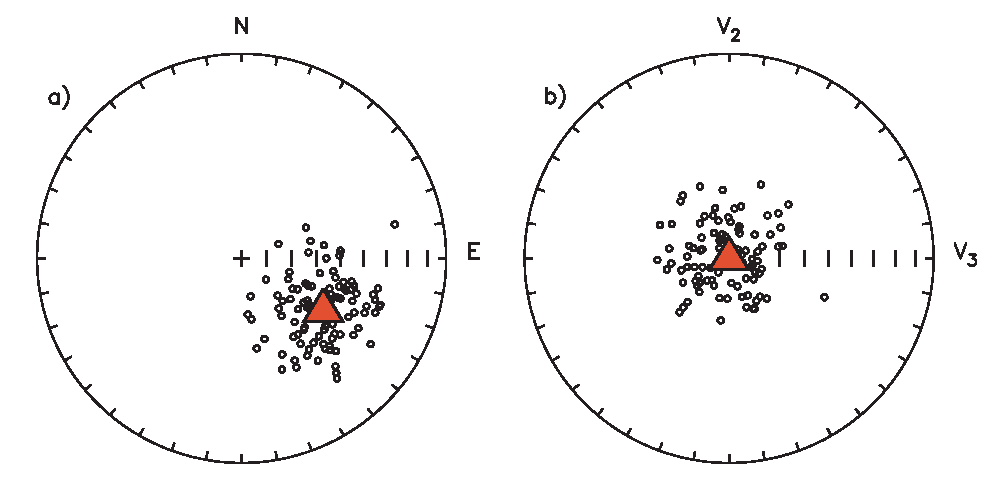
\includegraphics[width= 12.5 cm]{EPSfiles/fishrot.eps}
\caption{
Transformation of coordinates from a) geographic  to b) ``data'' coordinates.
 The
direction of the principal eigenvector $\V_1$ is shown by the triangle
in both plots.  [Figure redrawn from Tauxe, 1998.]}
\label{fig:fishrot}
\end{figure}


\begin{figure}[htb]
%\epsfxsize 12cm
%\centering \epsffile{EPSfiles/unexp.eps}
\centering  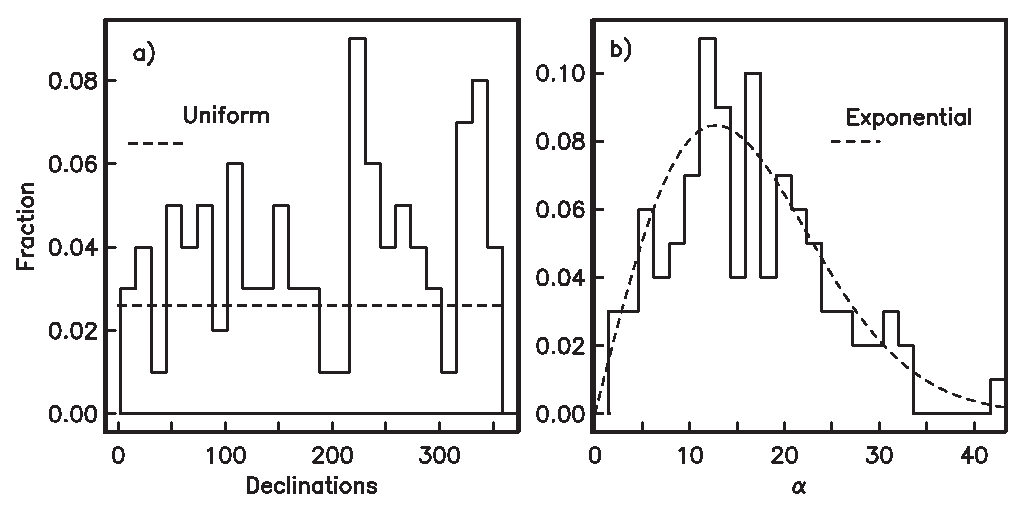
\includegraphics[width= 12 cm]{EPSfiles/unexp.eps}
\caption{
a) Declinations and b) co-inclinations ($\alpha$) from Figure 11.9. 
 Also shown are behaviors
expected for $D$ and $I$ from a Fisher distribution, i.e., declinations are
uniformly distributed while co-inclinations are exponentially distributed. 
[Figure from Tauxe, 1998.]}
\label{fig:unexp}
\end{figure}


\section {Is a given data set Fisher distributed?}
\label{sect:fishtests}

Clearly, the Fisher distribution allows powerful tests and this power lies
behind the popularity of paleomagnetism in solving geologic problems.  The
problem is that these tests require that the data be Fisher distributed.
How can we tell if a particular data set is Fisher distributed? 
 What do we do if the data are not Fisher distributed?  
These questions are addressed in  the rest of this chapter and the next one.  

\index{statistical tests!Fisher distribution}%
Let us now consider how to determine whether a given data set is Fisher
distributed.  
There are actually many ways of doing this.    There is a rather complete discussion
of  the problem in Fisher et al. (1987) and if you really want a complete treatment try the supplemental reading list at the end of this chapter.
\index{statistical tests!quantile-quantile}
The quantile-quantile (Q-Q) method described by Fisher et al. (1987) is fairly intuitive and works well.  We outline it briefly in the following. 


The idea behind the  {\it Q-Q}  method is to exploit the fact that declinations
in a Fisher distribution, when viewed about the mean, are spread around
the clock evenly -- there is  a uniform distribution of declinations.
Also, the inclinations (or rather the co-inclinations) are clustered
close to the mean and the frequency dies off exponentially away from the mean
direction.  

Therefore,
 the first  step  in testing for compatibility with a Fisher distribution is to transpose the data
such that the mean is the center of the distribution.  You can think
of this as rotating your head around to peer down the mean direction.
On an equal area projection, the center of the diagram will now be  the mean direction instead of the vertical.
In order to do this transformation, we first  
calculate the orientation matrix $\T$ of
the data and  the associated eigenvectors $\V_i$ and eigenvalues $\tau_i$
(Appendix~\ref{app:eigen} - in case you haven't read it yet, do so NOW). 
Substituting the direction cosines relating the geographic coordinate
system $\X$ to the coordinate system defined by $\V$, the eigenvectors, 
where $\X$ is the ``old'' and $\V$ is the ``new''
set of axes, we can transform the
coordinate system for a set of data from ``geographic'' coordinates
 (Figure~\ref{fig:fishrot}a) where the vertical axis is the center
of the diagram, to  the ``data'' coordinate system,
 (Figure~\ref{fig:fishrot}b)
where the principal eigenvector ($\V_1$) lies at the center of the
diagram, after transformation into ``data'' coordinates.  




Recalling that Fisher distributions are symmetrically disposed about the mean direction, but fall off exponentially away from that direction, let us compare the data from Figure~\ref{fig:fishrot} to the expected distributions
for a Fisher distribution with $\kappa = 20$ (Figure~\ref{fig:unexp}).
The data were generated  using the program \href{http://earthref.org/PmagPy/cookbook/#fisher.py}{\bf fisher.py} in the {\bf PmagPy} software distribution which relies on  the method 
outlined by 
\index{Fisher, N.I.}%
Fisher et al. (1987),  that
draws directions from a Fisher distribution with a specified $\kappa$.
We used  a $\kappa$ of 20,  and it
should come as no surprise that the data fit the expected
distribution rather well.  But how well is ``well'' and how can we tell
when a data set {\it fails} to be fit by a Fisher distribution? 
\begin{figure}[htb]
%\epsfxsize 11.25cm
%\centering \epsffile{EPSfiles/fishqq.eps}
\centering  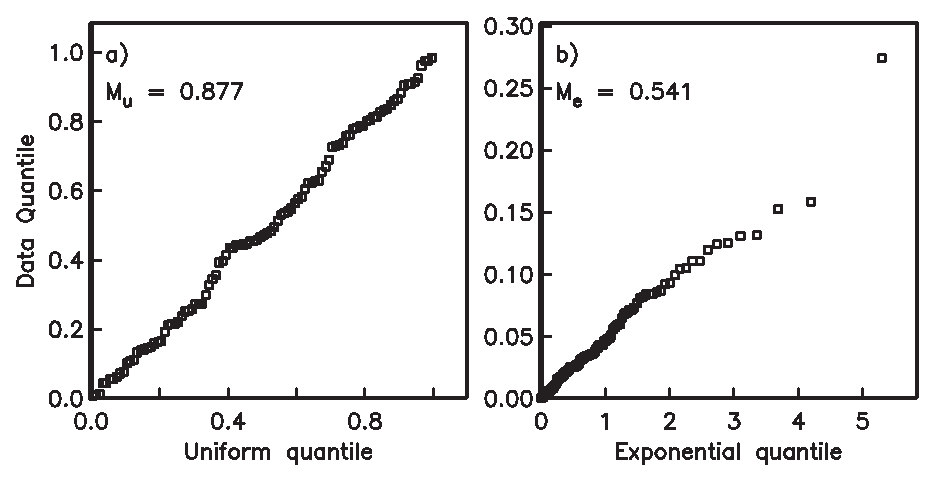
\includegraphics[width= 11.25 cm]{EPSfiles/fishqq.eps}
\caption{
a) Quantile-quantile plot of declinations (in data coordinates) from Figure
11.9  plotted against an assumed uniform distribution. b) Same for inclinations
plotted against an assumed exponential distribution. The data are Fisher distributed. [Figure from Tauxe, 1998.]}
\label{fig:fishqq}
\end{figure}

We wish to test whether the declinations are uniformly distributed
and whether the inclinations are exponentially distributed
 as required by the Fisher
distribution.  Plots such as those shown in Figure~\ref{fig:unexp} are not
as helpful for this purpose as a plot known as a 
\index{diagrams!quantile-quantile}%
\index{statistical tests!quantile-quantile!Fisher distribution}
{\it quantile-quantile} (Q-Q) diagram
\index{Fisher, N.I.}
(see Fisher et al., 1987).
In  a Q-Q plot, the data are graphed against the value expected from a
particular distribution. Data compatible with the chosen distribution plot along
a line.  The procedure for accomplishing  this is given in Appendix~\ref{app:qq}.  
In Figure~\ref{fig:fishqq}a, we plot the declinations from
Figure~\ref{fig:fishrot} (in data coordinates) against the  values
calculated assuming a uniform distribution and in Figure~\ref{fig:fishqq}b,
we plot the co-inclinations against
those calculated using an exponential distribution.
 As expected, the data plot along  lines.  Appendix~\ref{app:qq} outlines the calculation of two test statistics $M_u$ and $M_e$ which can be used to assess whether the data are uniformly or exponentially distributed respectively.   Neither of these  exceed the critical values.  




\vskip .5 in\noindent SUPPLEMENTAL READINGS: Fisher  et al. (1987),  Chapters 2--5. 





\section{Problems}

{\parindent 0pt \parskip 12pt 

Check the \href{http://earthref.org/PmagPy/cookbook/}{PmagPy website} for examples on how to use the {\bf PmagPy} programs in this problem set.  

{\bf Problem 1}

a) Use the program {\bf fishrot.py} to generate a Fisher distributed data set of $N=20$ data points, drawn from a true mean direction of $D = 12^{\circ}, I = 45^{\circ}$ and a $\kappa$ of  25.   Save these to a file called {\it prob1a.dat}.    (Use {\bf eqarea.py} to admire your handiwork.)   Hint:  use the Unix file redirect feature:   

\begin{verbatim}
% fishrot.py -n 20 -D 12  -I 45 -k 25 > ps11_prob1a.dat 
\end{verbatim}

Note that you can also do this from within a notebook using the '!' option in a code block:

\begin{verbatim}
fishrot.py -n 20 -D 12  -I 45 -k 25 > ps11_prob1a.dat 
\end{verbatim} 

As a challenge problem, you can use the function pmag.fshdev directly from the ipython notebook environment and plot it with the ipmag functions {\bf plot\_net} and  and {\bf plot\_di}.  

b) Write a program to read in {\it ps11\_prob1a.dat}  from a) and calculate the Fisher statistics of:  $\bar D, \bar I, k, \alpha_{95}, R$ and CSD.    

c) Now generate a second sample from the same distribution (just repeat the {\bf fishrot.py} command)  and put the second set of directions  in {\it prob1c.dat}.  These are two sets of directions drawn from the same distribution and certainly should share a common mean direction (logically).  But  do the two data sets  pass the simple Watson $F$ test for common mean direction?  [This test will fail 5\% of the time!]


d) Generate a third sample from a distribution with $D = 55^{\circ}, I = 60^{\circ}$ but the same $N$ and $\kappa$ and save it in {\it ps11\_prob1d.dat}.  Does this data set pass the $F$ test for common mean with the data in {\it prob1a.dat}?   Check your answer using the program {\bf watsonsF.py}.  

e)  An alternative method for testing for common mean with less restrictive assumptions uses  Watson's statistic $V_w$.  Use the program {\bf watsonsV.py} to  test {\it prob1a.dat} against {\it prob1c.dat} and {\it prob1d.dat}.  Do the answers  using $V_w$ agree with those using the $F$ test?     



{\bf Problem 2} 

a)  Generate a set of directions, drawn from a Fisher distribution with a true mean inclination of 70$^{\circ}$.   Calculate the Gaussian average of the  inclination data.  You can write your own script or use the {\bf PmagPy} program {\bf stats.py} for this.  [HINT: investigate the marvels of the Unix command {\bf awk}.  If you use a PC and think you do not have this, re-read the installation instructions for the {\bf PmagPy} software package -- there is a set of useful Unix utilities for you.] 

b) How does this compare with the average you calculate using your Fisher program (or {\bf gofish.py}).

c) Use the program {\bf incfish.py}, which does the inclination only calculation of $\bar I$.  Is this estimate closer to the Fisher estimate?   Or, you can call the {\bf pmag} module function {\bf doincfish} from within an IPython notebook.  

{\bf Problem 3}

a ) Unpack the Chapter\_11 datafile from the Datafiles archive (in the Essentials\_Examples folder in Datafiles that comes with the \href{http://earthref.org/PmagPy/cookbook}{\bf PmagPy} software package ).   You will find a file called {\it prob3a.dat}.   This has:   $D, I$, dip direction and dip from two limbs of the fold.    They are of both polarities.   Separate the data into normal and reverse polarity,  flip the reverse data over to their antipodes and calculate the Fisher statistics for the combined data set.   


b)     Use the program {\bf di\_tilt.py} to ``untilt'' the data (call {\bf pmag.dotilt} from an IPython notebook).   Repeat the procedure in a).     Would the two data sets pass a simple (McElhinny $F$ test) fold test?  

%{\bf Problem 4}
%
%a)  Refer to Problem 6 in Chapter 9 for help with importing data files into the MagIC format.  Someone has measured some more specimens from the same study that was the focus of that problem.  In the Chapter\_11 directory,  there is a directory named Problem4 with a sub-directory named MagIC.  From the command line,  fire up {\bf QuickMagIC.py} and choose this directory as your project directory.  Someone has already imported the orientation data, but you need to import the AF data from data file {\it ns\_a.mag} and the thermal demagnetization data in {\it ns\_t.mag} in the Chapter\_11 directory.    After importing both of these,  combine the measurements and interpret them using `Demag GUI' option.  
%
%b) Look at your interpretations at the site level as in Problem 6 in Chapter 9.  One of the sites (NS007) has a ``funny'' direction that you suspect might be an orientation error in the field of some kind.  Use the option Data Reduction/Upload$>$Check sample orientations to test several hypotheses about bad orientations.   Ignore all previous interpretations.     Find the name of the specimen by looking at the information in the command window and comparing it to the equal area plot.  Then type 'e' at the command window and (after hitting return) type in the specimen name.  You will see an equal area projection with the data as before, but now there is a small circle tracing out directions that would come if the orientation mark on the sample in the field was wrong (say if a stray mark was interpreted as the brass scratch).  There is also a triangle, if the arrow was marked the wrong direction (say out from the outcrop instead of in) and a $\Delta$ if someone read the wrong end of the compass in the field.  If any of these plots next to the rest of the directions, it may be reasonable to mark this sample orientation as ``bad'' and exclude it from the site mean.  So, select 'y' when asked and choosed ``bad mark'' as your excuse.  This remains a permanent part of the data, but specimens from this sample will not bother you again!  Quit the program and re-run the Assemble specimens option.  
%
%c)   Look at the specimen data (by site) with the equal area projections as in Problem 6 in Chapter 9.  Use the geographic coordinates when asked.  This time, select `Combine Lines \& Planes' as the confidence ellipses because you should have interpreted several of the specimens from Site NS016 as great circles.  

 }


